\documentclass{beamer}\usepackage[]{graphicx}\usepackage[]{color}
%% maxwidth is the original width if it is less than linewidth
%% otherwise use linewidth (to make sure the graphics do not exceed the margin)
\makeatletter
\def\maxwidth{ %
  \ifdim\Gin@nat@width>\linewidth
    \linewidth
  \else
    \Gin@nat@width
  \fi
}
\makeatother

\definecolor{fgcolor}{rgb}{1, 0.894, 0.769}
\newcommand{\hlnum}[1]{\textcolor[rgb]{0.824,0.412,0.118}{#1}}%
\newcommand{\hlstr}[1]{\textcolor[rgb]{1,0.894,0.71}{#1}}%
\newcommand{\hlcom}[1]{\textcolor[rgb]{0.824,0.706,0.549}{#1}}%
\newcommand{\hlopt}[1]{\textcolor[rgb]{1,0.894,0.769}{#1}}%
\newcommand{\hlstd}[1]{\textcolor[rgb]{1,0.894,0.769}{#1}}%
\newcommand{\hlkwa}[1]{\textcolor[rgb]{0.941,0.902,0.549}{#1}}%
\newcommand{\hlkwb}[1]{\textcolor[rgb]{0.804,0.776,0.451}{#1}}%
\newcommand{\hlkwc}[1]{\textcolor[rgb]{0.78,0.941,0.545}{#1}}%
\newcommand{\hlkwd}[1]{\textcolor[rgb]{1,0.78,0.769}{#1}}%
\let\hlipl\hlkwb

\usepackage{framed}
\makeatletter
\newenvironment{kframe}{%
 \def\at@end@of@kframe{}%
 \ifinner\ifhmode%
  \def\at@end@of@kframe{\end{minipage}}%
  \begin{minipage}{\columnwidth}%
 \fi\fi%
 \def\FrameCommand##1{\hskip\@totalleftmargin \hskip-\fboxsep
 \colorbox{shadecolor}{##1}\hskip-\fboxsep
     % There is no \\@totalrightmargin, so:
     \hskip-\linewidth \hskip-\@totalleftmargin \hskip\columnwidth}%
 \MakeFramed {\advance\hsize-\width
   \@totalleftmargin\z@ \linewidth\hsize
   \@setminipage}}%
 {\par\unskip\endMakeFramed%
 \at@end@of@kframe}
\makeatother

\definecolor{shadecolor}{rgb}{.97, .97, .97}
\definecolor{messagecolor}{rgb}{0, 0, 0}
\definecolor{warningcolor}{rgb}{1, 0, 1}
\definecolor{errorcolor}{rgb}{1, 0, 0}
\newenvironment{knitrout}{}{} % an empty environment to be redefined in TeX

\usepackage{alltt}
\usepackage{../371g-slides}
\usepackage{preview}
\title{Diagnostics \& Transformations 1}
\subtitle{Lecture 17}
\author{STA 371G}
\IfFileExists{upquote.sty}{\usepackage{upquote}}{}
\begin{document}
  
  

  \frame{\maketitle}

  % Show outline at beginning of each section
  \AtBeginSection[]{ 
    \begin{frame}<beamer>
      \tableofcontents[currentsection]
    \end{frame}
  }

  %%%%%%% Slides start here %%%%%%%

  \begin{darkframes}
    
    
    \begin{frame}
      \fontsize{9}{9}\selectfont
      Predicting the fuel economy (miles per gallon) for different car models of the 70s.
      
      \begin{center}
        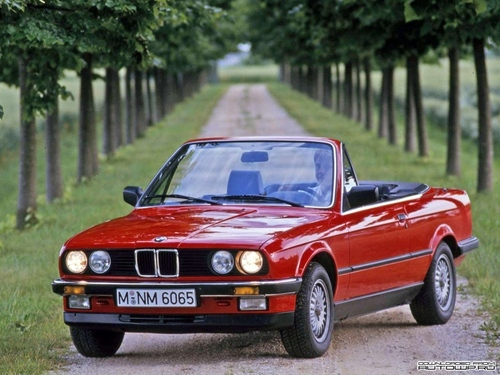
\includegraphics[width=2.8in]{bmw} \\
      \end{center} \pause
      
      Regression assumptions:
      \begin{columns}[onlytextwidth]
        \column{.5\textwidth}
          \begin{itemize}
            \item Linearity
            \item Independent errors
          \end{itemize}
        \column{.5\textwidth}
          \begin{itemize}
            \item Normally distributed errors
            \item Equal Variance (Homoscedasticity)
          \end{itemize}
      \end{columns}
    \end{frame}
    
    
    
    \begin{frame}[fragile]{Predicting MPG from Horsepower}
    \fontsize{9}{9}\selectfont
\begin{knitrout}
\definecolor{shadecolor}{rgb}{0.137, 0.137, 0.137}\begin{kframe}
\begin{alltt}
  \hlstd{model} \hlkwb{<-} \hlkwd{lm}\hlstd{(MPG} \hlopt{~} \hlstd{HP,} \hlkwc{data}\hlstd{=auto_mpg)}
  \hlkwd{summary}\hlstd{(model)}
\end{alltt}
\begin{verbatim}

Call:
lm(formula = MPG ~ HP, data = auto_mpg)

Residuals:
     Min       1Q   Median       3Q      Max 
-13.5710  -3.2592  -0.3435   2.7630  16.9240 

Coefficients:
             Estimate Std. Error t value Pr(>|t|)    
(Intercept) 39.935861   0.717499   55.66   <2e-16 ***
HP          -0.157845   0.006446  -24.49   <2e-16 ***
---
Signif. codes:  0 '***' 0.001 '**' 0.01 '*' 0.05 '.' 0.1 ' ' 1

Residual standard error: 4.906 on 390 degrees of freedom
Multiple R-squared:  0.6059,	Adjusted R-squared:  0.6049 
F-statistic: 599.7 on 1 and 390 DF,  p-value: < 2.2e-16
\end{verbatim}
\end{kframe}
\end{knitrout}
    \end{frame}
    
    
    
    \begin{frame}[fragile]
    \fontsize{9}{9}\selectfont
\begin{knitrout}
\definecolor{shadecolor}{rgb}{0.137, 0.137, 0.137}\begin{kframe}
\begin{alltt}
  \hlkwd{plot}\hlstd{(model}\hlopt{$}\hlstd{fitted.values,} \hlkwd{resid}\hlstd{(model),} \hlkwc{col}\hlstd{=}\hlstr{'green'}\hlstd{)}
\end{alltt}
\end{kframe}
\input{/tmp/figures/unnamed-chunk-3-1.tikz}

\end{knitrout}
      \pause
      What's wrong here?
      \pause
      \begin{itemize}
      \item      The trend in the residuals implies linearity issues.
      \item The ``funnel'' implies equal variance issues.
    \end{itemize}	   
      
    \end{frame}
    
    
    
    \begin{frame}[fragile]{Addressing the linearity issue}
      \fontsize{9}{9}\selectfont
        The relation between MPG and horsepower does not seem to be linear.
\begin{knitrout}
\definecolor{shadecolor}{rgb}{0.137, 0.137, 0.137}\begin{kframe}
\begin{alltt}
  \hlkwd{plot}\hlstd{(auto_mpg}\hlopt{$}\hlstd{HP, auto_mpg}\hlopt{$}\hlstd{MPG,} \hlkwc{col}\hlstd{=}\hlstr{'green'}\hlstd{,}
       \hlkwc{xlab}\hlstd{=}\hlstr{'Horsepower'}\hlstd{,} \hlkwc{ylab}\hlstd{=}\hlstr{'MPG'}\hlstd{)}
  \hlkwd{abline}\hlstd{(model,} \hlkwc{col}\hlstd{=}\hlstr{'cyan'}\hlstd{,} \hlkwc{lwd}\hlstd{=}\hlnum{3}\hlstd{)}
\end{alltt}
\end{kframe}
\input{/tmp/figures/unnamed-chunk-4-1.tikz}

\end{knitrout}
    \end{frame}
    
    
    
    \begin{frame}[fragile]{Addressing the linearity issue}
      %\fontsize{9}{9}\selectfont
      \begin{center}
        If we could horizontally shift the data on the far right towards the left, the plot would look more linear.
        \bigskip \pause
        
        So let's predict the MPG of a car not from the horsepower, but from a ``transformation'' of the horsepower. \pause
        \bigskip
        
        For example, the relation between MPG and HP is not linear, but the one between MPG and $\sqrt{\text{HP}}$ could be!
      \end{center}
    
    \end{frame}
    
    
    
    
    \begin{frame}[fragile]{Addressing the linearity issue}
      \fontsize{9}{9}\selectfont
\begin{knitrout}
\definecolor{shadecolor}{rgb}{0.137, 0.137, 0.137}\begin{kframe}
\begin{alltt}
  \hlstd{auto_mpg}\hlopt{$}\hlstd{HP_sqrt} \hlkwb{<-} \hlkwd{sqrt}\hlstd{(auto_mpg}\hlopt{$}\hlstd{HP)}
  \hlkwd{plot}\hlstd{(auto_mpg}\hlopt{$}\hlstd{HP_sqrt, auto_mpg}\hlopt{$}\hlstd{MPG,} \hlkwc{col}\hlstd{=}\hlstr{'green'}\hlstd{,}
       \hlkwc{xlab}\hlstd{=}\hlstr{'Squareroot of Horsepower'}\hlstd{,} \hlkwc{ylab}\hlstd{=}\hlstr{'MPG'}\hlstd{)}
\end{alltt}
\end{kframe}
\input{/tmp/figures/unnamed-chunk-5-1.tikz}

\end{knitrout}
     \end{frame}  
    
    
      
    
    
    
    \begin{frame}[fragile]{Addressing the linearity issue}
      \fontsize{9}{9}\selectfont
      
        It indeed seems a bit better. Notice the change in the range of the horizontal axis. \pause
      
        It has changed from [49,225] to [7,15]. The shift is larger for the data on the far right. 
      
\begin{knitrout}
\definecolor{shadecolor}{rgb}{0.137, 0.137, 0.137}\begin{kframe}
\begin{alltt}
 \hlkwd{plot}\hlstd{(auto_mpg}\hlopt{$}\hlstd{HP, auto_mpg}\hlopt{$}\hlstd{HP_sqrt,} \hlkwc{col}\hlstd{=}\hlstr{'green'}\hlstd{,}
     \hlkwc{xlab}\hlstd{=}\hlstr{'Horsepower'}\hlstd{,} \hlkwc{ylab}\hlstd{=}\hlstr{'Squareroot of Horsepower'}\hlstd{)}
\end{alltt}
\end{kframe}
\input{/tmp/figures/unnamed-chunk-6-1.tikz}

\end{knitrout}
    \end{frame}
  
  
  
    \begin{frame}[fragile]{Addressing the linearity issue}
      \fontsize{9}{9}\selectfont
\begin{knitrout}
\definecolor{shadecolor}{rgb}{0.137, 0.137, 0.137}\begin{kframe}
\begin{alltt}
  \hlstd{model2} \hlkwb{<-} \hlkwd{lm}\hlstd{(MPG} \hlopt{~} \hlstd{HP_sqrt,} \hlkwc{data}\hlstd{=auto_mpg)}
  \hlkwd{summary}\hlstd{(model2)}
\end{alltt}
\begin{verbatim}

Call:
lm(formula = MPG ~ HP_sqrt, data = auto_mpg)

Residuals:
     Min       1Q   Median       3Q      Max 
-13.9768  -3.2239  -0.2252   2.6881  16.1411 

Coefficients:
            Estimate Std. Error t value Pr(>|t|)    
(Intercept)   58.705      1.349   43.52   <2e-16 ***
HP_sqrt       -3.503      0.132  -26.54   <2e-16 ***
---
Signif. codes:  0 '***' 0.001 '**' 0.01 '*' 0.05 '.' 0.1 ' ' 1

Residual standard error: 4.665 on 390 degrees of freedom
Multiple R-squared:  0.6437,	Adjusted R-squared:  0.6428 
F-statistic: 704.6 on 1 and 390 DF,  p-value: < 2.2e-16
\end{verbatim}
\end{kframe}
\end{knitrout}
    \end{frame}
    
    
    \begin{frame}[fragile]
    \fontsize{9}{9}\selectfont
\begin{knitrout}
\definecolor{shadecolor}{rgb}{0.137, 0.137, 0.137}\begin{kframe}
\begin{alltt}
  \hlkwd{plot}\hlstd{(model2}\hlopt{$}\hlstd{fitted.values,} \hlkwd{resid}\hlstd{(model2),} \hlkwc{col}\hlstd{=}\hlstr{'green'}\hlstd{)}
\end{alltt}
\end{kframe}
\input{/tmp/figures/unnamed-chunk-8-1.tikz}

\end{knitrout}
      The trend flattened a bit. \pause
      
      Can we do better? Let's try some other transformation.
    \end{frame}
    
    
    
    \begin{frame}[fragile]{Logarithmic transformation}
    %\fontsize{9}{9}\selectfont
      \begin{center}
        One of the most common transformations is the logarithmic transformation with base $e$ (natural logarithm). \bigskip \pause
        
        $e=2.7182818284\ldots$ \bigskip \pause
        
        $e^2 = 7.389$ \bigskip \pause
        
        $\log(e^2) = 2$ \bigskip \pause
        
        In general:
        
        $y=e^x \qquad\longleftrightarrow\qquad \log y = x$.
      
      \end{center}
        
    \end{frame}
    
    
    \begin{frame}[fragile]{Logarithmic transformation}
      \fontsize{9}{9}\selectfont
\begin{knitrout}
\definecolor{shadecolor}{rgb}{0.137, 0.137, 0.137}\begin{kframe}
\begin{alltt}
  \hlstd{auto_mpg}\hlopt{$}\hlstd{HP_ln} \hlkwb{<-} \hlkwd{log}\hlstd{(auto_mpg}\hlopt{$}\hlstd{HP)}
  \hlkwd{plot}\hlstd{(auto_mpg}\hlopt{$}\hlstd{HP, auto_mpg}\hlopt{$}\hlstd{HP_ln,} \hlkwc{col}\hlstd{=}\hlstr{'green'}\hlstd{,}
      \hlkwc{xlab}\hlstd{=}\hlstr{'Horsepower'}\hlstd{,} \hlkwc{ylab}\hlstd{=}\hlstr{'Log of Horsepower'}\hlstd{)}
\end{alltt}
\end{kframe}
\input{/tmp/figures/unnamed-chunk-9-1.tikz}

\end{knitrout}
     \end{frame}  
    
    
    
    
    \begin{frame}[fragile]{Logarithmic transformation}
      \fontsize{9}{9}\selectfont
\begin{knitrout}
\definecolor{shadecolor}{rgb}{0.137, 0.137, 0.137}\begin{kframe}
\begin{alltt}
  \hlkwd{plot}\hlstd{(auto_mpg}\hlopt{$}\hlstd{HP_ln, auto_mpg}\hlopt{$}\hlstd{MPG,} \hlkwc{col}\hlstd{=}\hlstr{'green'}\hlstd{,}
       \hlkwc{xlab}\hlstd{=}\hlstr{'Log of Horsepower'}\hlstd{,} \hlkwc{ylab}\hlstd{=}\hlstr{'MPG'}\hlstd{)}
\end{alltt}
\end{kframe}
\input{/tmp/figures/unnamed-chunk-10-1.tikz}

\end{knitrout}
    \end{frame}
    

    \begin{frame}[fragile]
      \fontsize{9}{9}\selectfont
\begin{knitrout}
\definecolor{shadecolor}{rgb}{0.137, 0.137, 0.137}\begin{kframe}
\begin{alltt}
  \hlstd{model3} \hlkwb{<-} \hlkwd{lm}\hlstd{(MPG} \hlopt{~} \hlstd{HP_ln,} \hlkwc{data}\hlstd{=auto_mpg)}
  \hlkwd{summary}\hlstd{(model3)}
\end{alltt}
\begin{verbatim}

Call:
lm(formula = MPG ~ HP_ln, data = auto_mpg)

Residuals:
     Min       1Q   Median       3Q      Max 
-14.2299  -2.7818  -0.2322   2.6661  15.4695 

Coefficients:
            Estimate Std. Error t value Pr(>|t|)    
(Intercept) 108.6997     3.0496   35.64   <2e-16 ***
HP_ln       -18.5822     0.6629  -28.03   <2e-16 ***
---
Signif. codes:  0 '***' 0.001 '**' 0.01 '*' 0.05 '.' 0.1 ' ' 1

Residual standard error: 4.501 on 390 degrees of freedom
Multiple R-squared:  0.6683,	Adjusted R-squared:  0.6675 
F-statistic: 785.9 on 1 and 390 DF,  p-value: < 2.2e-16
\end{verbatim}
\end{kframe}
\end{knitrout}
    \end{frame}
    
    
    \begin{frame}[fragile]
\begin{knitrout}
\definecolor{shadecolor}{rgb}{0.137, 0.137, 0.137}\begin{kframe}
\begin{alltt}
  \hlkwd{plot}\hlstd{(model3}\hlopt{$}\hlstd{fitted.values,} \hlkwd{resid}\hlstd{(model3),} \hlkwc{col}\hlstd{=}\hlstr{'green'}\hlstd{)}
\end{alltt}
\end{kframe}
\input{/tmp/figures/unnamed-chunk-12-1.tikz}

\end{knitrout}
      The trend flattened even more. 
    \end{frame}


    \begin{frame}[fragile]{Transforming a Predictor}
      \begin{center}
        It is equivalent to ``cutting the distribution of $X$ into vertical slices and changing the spacing of the slices.'' \bigskip \pause
        
        It does not affect the vertical locations of the data (MPG did not change!). \bigskip \pause
        
        When the nonlinearity is the biggest issue in the model, transforming the predictor is a good start. \bigskip \pause
        
        Finding the right transformation is a bit of art, field knowledge and trial and error.
        
      \end{center}
      
      \lc
    
    \end{frame}
    
    \begin{frame}{Transforming a Predictor}

      \begin{center}
        \begin{tabular}{lll}
          \hline
          $X$ & $\sqrt{X}$ & $\log X$ \\
          \hline
          1 & $1$ & $0$ \\
          10 & $3.16$ & $2.3$ \\
          100 & $10$ & $4.61$ \\
          1000 & $31.62$ & $6.91$ \\
          10000 & $100$ & $9.21$ \\
          100000 & $316.23$ & $11.51$ \\
          \hline
        \end{tabular}
      \end{center}
    \end{frame}
    
    
    \begin{frame}[fragile]{Addressing the equal variance issue}
      \begin{columns}[onlytextwidth]
        \column{.5\textwidth}
          \begin{itemize}[<+->]
            \item The (unexplained) variance in the response is higher in some regions.
            \item Remember how log-transformation shrinks larger numbers more than it shrinks smaller numbers.
            \item Log-transformation of the response often helps with fixing heteroscedasticity (and non-normality)!
          \end{itemize}
        \column{.5\textwidth}
\begin{knitrout}
\definecolor{shadecolor}{rgb}{0.137, 0.137, 0.137}
\input{/tmp/figures/unnamed-chunk-14-1.tikz}

\end{knitrout}
      \end{columns}
    \end{frame}
  
  
  
    \begin{frame}[fragile]
      \fontsize{9}{9}\selectfont
\begin{knitrout}
\definecolor{shadecolor}{rgb}{0.137, 0.137, 0.137}\begin{kframe}
\begin{alltt}
  \hlstd{auto_mpg}\hlopt{$}\hlstd{MPG_ln} \hlkwb{<-} \hlkwd{log}\hlstd{(auto_mpg}\hlopt{$}\hlstd{MPG)}
  \hlstd{model4} \hlkwb{<-} \hlkwd{lm}\hlstd{(MPG_ln} \hlopt{~} \hlstd{HP_ln,} \hlkwc{data}\hlstd{=auto_mpg)}
  \hlkwd{summary}\hlstd{(model4)}
\end{alltt}
\begin{verbatim}

Call:
lm(formula = MPG_ln ~ HP_ln, data = auto_mpg)

Residuals:
    Min      1Q  Median      3Q     Max 
-0.6523 -0.1218  0.0079  0.1163  0.6373 

Coefficients:
            Estimate Std. Error t value Pr(>|t|)    
(Intercept)   6.9606     0.1215    57.3   <2e-16 ***
HP_ln        -0.8418     0.0264   -31.9   <2e-16 ***
---
Signif. codes:  0 '***' 0.001 '**' 0.01 '*' 0.05 '.' 0.1 ' ' 1

Residual standard error: 0.18 on 390 degrees of freedom
Multiple R-squared:  0.723,	Adjusted R-squared:  0.722 
F-statistic: 1.02e+03 on 1 and 390 DF,  p-value: <2e-16
\end{verbatim}
\end{kframe}
\end{knitrout}
    \end{frame}
    
    
    \begin{frame}[fragile]%{Addressing the equal variance issues}
      \fontsize{9}{9}\selectfont
\begin{knitrout}
\definecolor{shadecolor}{rgb}{0.137, 0.137, 0.137}\begin{kframe}
\begin{alltt}
  \hlkwd{plot}\hlstd{(auto_mpg}\hlopt{$}\hlstd{HP_ln, auto_mpg}\hlopt{$}\hlstd{MPG_ln,} \hlkwc{col}\hlstd{=}\hlstr{'green'}\hlstd{,}
       \hlkwc{xlab}\hlstd{=}\hlstr{'Log of Horsepower'}\hlstd{,} \hlkwc{ylab}\hlstd{=}\hlstr{'Log of MPG'}\hlstd{)}
  \hlkwd{abline}\hlstd{(model4,} \hlkwc{col}\hlstd{=}\hlstr{'cyan'}\hlstd{,} \hlkwc{lwd}\hlstd{=}\hlnum{3}\hlstd{)}
\end{alltt}
\end{kframe}
\input{/tmp/figures/unnamed-chunk-16-1.tikz}

\end{knitrout}
    \end{frame}
    
    
    \begin{frame}[fragile]
      Beautiful!
\begin{knitrout}
\definecolor{shadecolor}{rgb}{0.137, 0.137, 0.137}\begin{kframe}
\begin{alltt}
  \hlkwd{plot}\hlstd{(model4}\hlopt{$}\hlstd{fitted.values,} \hlkwd{resid}\hlstd{(model4),} \hlkwc{col}\hlstd{=}\hlstr{'green'}\hlstd{)}
\end{alltt}
\end{kframe}
\input{/tmp/figures/unnamed-chunk-17-1.tikz}

\end{knitrout}
    \end{frame}
  
    \begin{frame}{Look how awesome our models are getting}

      \begin{center}
        \begin{tabular}{llll}
          Predictor ($X$) & Response ($Y$) & $R^2$ & Residual SE \\
          \hline
          $\text{HP}$ & $\text{MPG}$ & 0.61 & 4.91 \\
          $\sqrt{\text{HP}}$ & $\text{MPG}$ & 0.64  & 4.66 \\
          $\log\text{HP}$ & $\text{MPG}$ & 0.67 & 4.5 \\
          $\log\text{HP}$ & $\log\text{MPG}$ & 0.72 & 0.18 \\
        \end{tabular}
      \end{center}
    \end{frame}
  
  
  
  
    \begin{frame}[fragile]{Interpretation of $\beta$ values}

      \begin{center} 
        The model before the transformations was:
        
        \[
          \widehat{\text{MPG}} = 39.94 - 0.16 \cdot\text{HP}
        \] 

        \bigskip \pause
        
        The interpretation of $- 0.16$ is ``for each unit of increase in the horsepower, the MPG estimate reduces by $ 0.16$''.
        \bigskip \pause
        
        \alert{After transforming the predictor or the response, this interpretation does not hold!}
      
      \end{center}
    \end{frame}
  
  
  
  \begin{frame}[fragile]{Interpretation of $\beta$ values}

      \begin{center} 
        When the square root of HP is used: \bigskip
        
        \[
        \widehat{\text{MPG}} = 58.71 
        - 3.5 \cdot\sqrt{\text{HP}}        
        \] \bigskip \pause
        
        The interpretation of $- 3.5$ is ``for each unit of increase \alert{in the square root of the horsepower}, the MPG estimate reduces by $ 3.5$''.
        
        \lc
        
      
      \end{center}
    \end{frame}
  
  
  \begin{frame}[fragile]{Interpretation of $\beta$ values}

      \begin{center} 
        Similarly, in the following model: \bigskip
        
        \[
        \widehat{\text{MPG}} = 108.7 
        - 18.58 \cdot\log{\text{HP}}
        \] \bigskip \pause
        
        The interpretation of $- 18.58$ is ``for each unit of increase \alert{in the natural logarithm of the horsepower}, the MPG estimate reduces by $ 18.58$''.
        
        \lc
        
      
      \end{center}
    \end{frame}

  
  
  
    \begin{frame}[fragile]{Transformation strategy}
      \begin{itemize}[<+->]
        \item If the model has two or three of the equal variance, normality and linearity issues, try transforming $Y$.
        \item Transforming the response often fixes nonlinearity in addition to fixing normality and equal variance issues.
        \item After transforming the response, if the nonlinearity is not fixed, try transforming the predictor(s) as well.
        \item There is no rule for which transformations will work in all cases; trial and error may be required.
        \item Remember, the interpretations of the coefficients will change after you transform one or more variables!
      \end{itemize}
    \end{frame}
  

  \end{darkframes}

  \end{document}
